% replace all text with your own text.
% in this template few examples are mention
\chapter{Methodology}
\label{ch:method} % Label for method chapter

\section{Dataset Overview and Data Exploration}

The MNIST dataset serves as a fundamental benchmark in the field of machine learning research, particularly in tasks related to image classification and recognition. This dataset consists of a collection of grayscale images of handwritten digits (0-9), each accompanied by its corresponding label indicating the digit it represents. Researchers widely utilize the MNIST dataset to evaluate the efficacy of various algorithms and techniques for digit recognition tasks.

The MNIST dataset comprises 70,000 grayscale images, divided into a training set of 60,000 images and a test set of 10,000 images. Each image is a 28x28 pixel square, resulting in a total of 784 pixels per image. These pixels represent the grayscale intensity, ranging from 0 (black) to 255 (white). Additionally, each image is associated with a label, providing ground truth information about the digit depicted in the image.

\begin{table}[htbp]
\centering
\caption{Dataset Attributes and Data Types for MNIST Dataset}
\label{tab:mnist_attributes}
\begin{tabular}{@{}lll@{}}
\toprule
\textbf{Attribute} & \textbf{Description}            & \textbf{Data Type} \\ \midrule
Image              & Handwritten digit image        & Image (28x28 pixels, grayscale) \\
Label              & Digit label                    & Integer (0 to 9) \\ 
\bottomrule
\end{tabular}
\end{table}

\subsection{Loading the Dataset} 

The MNIST dataset will be retrieved from reputable sources, such as TensorFlow or PyTorch libraries, ensuring data integrity and consistency. Both the training and testing datasets will be loaded into the research environment for further exploration.

\subsection{Visualizing Sample Images}

A random selection of sample images from the dataset will be visualized to gain insights into the characteristics of handwritten digits. These images will be displayed alongside their corresponding labels, facilitating an understanding of the dataset's content.

\begin{figure}[htbp]
  \centering
  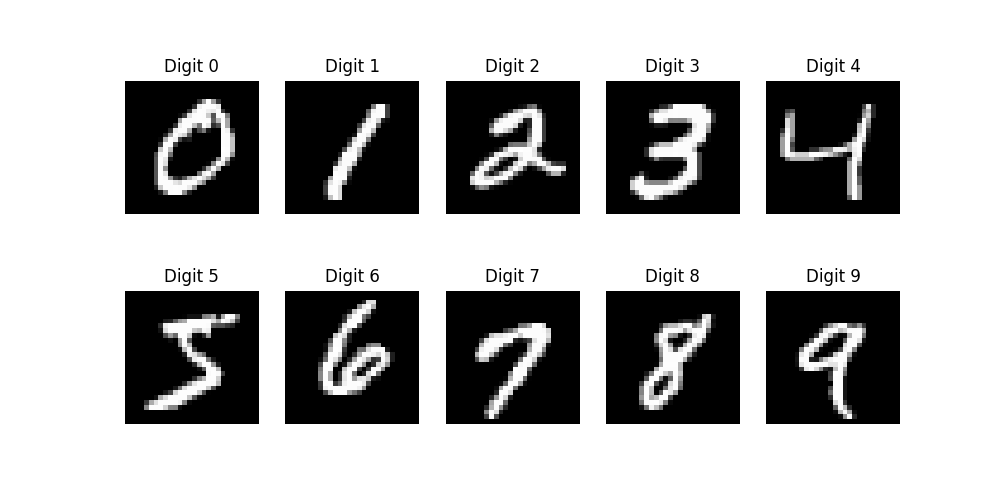
\includegraphics[width=1.0\textwidth]{figures/mnist_images.png}
  \caption{MNIST Example Images}
  \label{fig:mnist_image}
\end{figure}

\subsection{Exploring Label Distribution}

\begin{figure}[htbp]
  \centering
  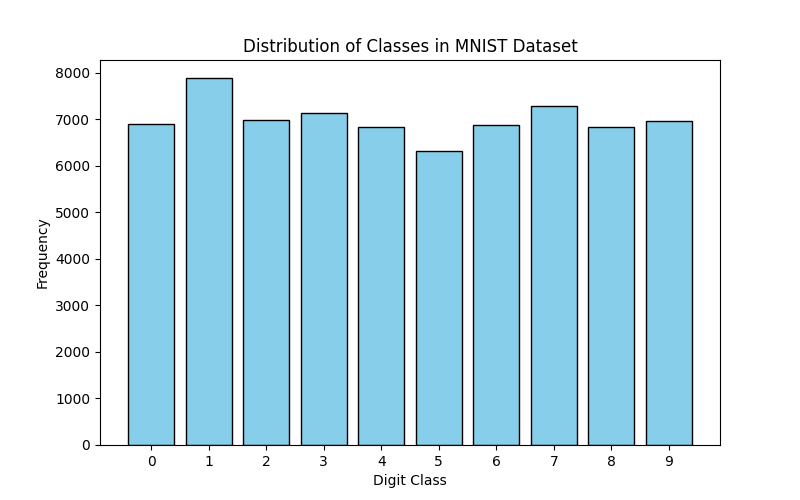
\includegraphics[width=0.7\textwidth]{figures/data_distribution.png}
  \caption{Distribution of Classes in MNIST Dataset}
  \label{fig:data_distribution}
\end{figure}

A histogram is plotted to visualize the distribution of digit labels within the training set. It is imperative to ensure that the dataset exhibits balanced label distributions, with a similar number of samples for each digit class.

\section{Data Preprocessing}

\subsection{Flatten the image data}

In the MNIST dataset, each image represents a handwritten digit and is initially structured as a 2-dimensional array (28x28 pixels). However, most machine learning algorithms, including neural networks, require input data to be in a flat, one-dimensional format. Flattening the image data involves reshaping each image into a single vector by stacking the rows of pixels one after another. This transformation simplifies the representation of the image data and allows us to treat each pixel as a separate feature. Flattening the data ensures compatibility with various machine learning models and facilitates efficient computation during training and prediction processes.

\subsection{Normalize the pixel values:}

The pixel values in the MNIST dataset represent the intensity of grayscale pixels ranging from 0 to 255. Normalizing the pixel values involves scaling them to a standard range, typically between 0 and 1 or -1 and 1. Normalization helps in stabilizing and speeding up the training process of machine learning models. It prevents certain features from dominating others due to differences in scale, thereby improving the convergence of optimization algorithms. Moreover, normalization ensures that the model's performance is not sensitive to the absolute values of the input features, making it more robust and generalizable across different datasets.

\subsection{Split the dataset into training and testing sets:}

Splitting the dataset into training and testing sets is crucial for evaluating the performance of machine learning models. The training set is used to train the model, while the testing set is used to evaluate its performance on unseen data. Additionally, it is common practice to further split the training set into a training subset and a validation set. The training subset is used for actual model training, while the validation set is used to tune hyperparameters and monitor the model's performance during training. This split helps prevent overfitting by providing an independent dataset for model evaluation and parameter tuning. Overall, splitting the dataset ensures that the model's performance estimates are reliable and generalizable to unseen data.


\subsection{Adding Noise to MNIST Images}

The add noise function provides a convenient way to induce varied levels of Gaussian noise into the MNIST dataset. This function takes two parameters: images, which represents the array of MNIST images, and noise level, which specifies the variance of the Gaussian noise to be added. The higher the noise level, the more intense the noise added to the images.

Internally, the function generates Gaussian noise with the specified variance and adds it to the input images. It ensures that the pixel values remain within the valid range of [0, 255] by clipping the values after adding noise.
By incorporating this function into the preprocessing pipeline, we can create augmented versions of the MNIST dataset with different levels of noise. These augmented datasets can help improve the model's performance, especially in scenarios where the input data may exhibit variability or uncertainty.

\section{Model Implementation}
This is the critical step where we build the model to predict handwritten digits.

\subsection{Convolutional Neural Network}

It is used for accurately classifying handwritten digits in the MNIST dataset due to their ability to effectively capture spatial patterns within images.

\begin{algorithm}
    \caption{Handwritten Digit Classification using Convolutional Neural Networks}
    \begin{algorithmic}[1]
        \Require Images $X$ and corresponding labels $y$ for training data
        \Ensure Performance metrics including accuracy, confusion matrix, precision, recall, and F1-score
        \State Create a convolutional neural network model with default architecture
        \State Train the model using the training data (images $X$ and labels $y$)
        \State Evaluate the model's performance metrics such as accuracy, confusion matrix, precision, recall, and F1-score
        \State Predict the labels for the testing data using the trained model
        \State Assess the model's performance on the testing data
        \State Calculate the performance metrics including accuracy, confusion matrix, precision, recall, and F1-score.
    \end{algorithmic}
\end{algorithm}

\subsection{Handwritten Digit Classification using Denoising Auto-encoder}

It is employed for enhancing the robustness of feature extraction in MNIST dataset classification tasks by reconstructing clean images from noisy inputs.


\begin{algorithm}
    \caption{Denoising Autoencoder}
        \begin{algorithmic}[1]
            \Require Noisy images $X_{\text{noisy}}$ and clean images $X_{\text{clean}}$ for training data
            \Ensure Reconstructed clean images from noisy inputs
            \State Create a denoising autoencoder model with encoder and decoder architecture
            \State Train the denoising autoencoder using the noisy images $X_{\text{noisy}}$ and their corresponding clean images $X_{\text{clean}}$
            \State Evaluate the performance of the denoising autoencoder by measuring reconstruction error
            \State Use the trained denoising autoencoder to reconstruct clean images from noisy inputs
        \end{algorithmic}
\end{algorithm}

\subsection{Hyperparameter Tuning with GridSearchCV}
Hyperparameter tuning is a critical step in optimizing the performance of Convolutional Neural Networks (CNN) and Denoising Autoencoders (DAE). By fine-tuning hyperparameters, we aim to identify the optimal configuration that maximizes the performance metrics of these models. One popular approach for hyperparameter tuning is GridSearchCV, which systematically explores a predefined grid of hyperparameter values to find the best combination for the given problem.

\subsubsection{Grid Search}
Grid Search involves specifying a set of hyperparameter values for each hyperparameter of the model. These values form a grid, and the model is trained and evaluated for each combination of hyperparameter values. The performance of the model is then assessed using cross-validation, typically employing techniques such as k-fold cross-validation.By leveraging GridSearchCV, we can effectively fine-tune the hyperparameters of CNNs and DAEs, optimizing their performance for tasks such as image classification and denoising. This systematic approach helps us identify the most suitable hyperparameter values, ultimately leading to improved model performance and generalization.

\subsubsection{Hyperparameter Tuning for CNN}
Hyperparameter tuning for Convolutional Neural Networks (CNNs) is a critical step in optimizing their performance for image classification tasks. GridSearchCV is a popular technique used for this purpose. It involves systematically exploring a predefined grid of hyperparameters and selecting the combination that yields the best performance on a validation set. This process helps identify the optimal values for hyperparameters such as learning rate, batch size, number of filters, kernel size, and dropout rate, ultimately leading to improved accuracy and generalization of the CNN model.
 
\begin{algorithm}
    \caption{Hyperparameter Tuning for CNN using GridSearchCV}
    \begin{algorithmic}[1]
        \Require CNN model architecture, hyperparameter grid
        \Ensure Optimized hyperparameters for the CNN model
        \State Define a grid of hyperparameters to be tuned
        \State Initialize GridSearchCV with the CNN model and hyperparameter grid
        \State Perform grid search with cross-validation to evaluate each hyperparameter combination
        \State Identify the optimal hyperparameters based on the chosen performance metric (e.g., accuracy)
        \State Train the CNN model using the optimal hyperparameters
        \State \textbf{return} Optimized hyperparameters for the CNN model
    \end{algorithmic}
\end{algorithm}

\subsubsection{Hyperparameter Tuning for DAE}
Hyperparameter tuning for Denoising Autoencoders (DAEs) using GridSearchCV is crucial for enhancing their performance in tasks such as image denoising and feature extraction. GridSearchCV systematically explores a predefined grid of hyperparameters, including parameters like learning rate, batch size, number of layers, activation functions, and regularization techniques. By evaluating different combinations of these hyperparameters through cross-validation, GridSearchCV helps identify the optimal configuration that maximizes the denoising performance of the DAE. This process ensures that the DAE model is fine-tuned to achieve better denoising results and robustness to noise in input data.

\begin{algorithm}
    \caption{Hyperparameter Tuning for Denoising Autoencoder using GridSerachCV}
    \begin{algorithmic}[1]
        \Require Noisy MNIST images $\mathbf{X}$, clean MNIST images $\mathbf{Y}$
        \Ensure Trained denoising autoencoder model $\mathcal{M}$
        \State Define the architecture of the denoising autoencoder model $\mathcal{M}$, including encoder and decoder layers
        \State Compile the denoising autoencoder model $\mathcal{M}$ with appropriate loss function and optimizer
        \State Generate noisy images $\tilde{\mathbf{X}}$ by adding random noise to the clean images $\mathbf{Y}$
        \State Train the denoising autoencoder model $\mathcal{M}$ using the noisy images $\tilde{\mathbf{X}}$ and the corresponding clean images $\mathbf{Y}$
        \State \textbf{return} Trained denoising autoencoder model $\mathcal{M}$
    \end{algorithmic}
\end{algorithm}

\section{Summary}
The methodology section outlines the research approach, beginning with an overview of the MNIST dataset and exploratory data analysis. It covers data preprocessing steps like flattening and normalizing image data, along with splitting the dataset. Model implementation details for Convolutional Neural Networks (CNNs) and Denoising Autoencoders (DAEs) are provided, emphasizing their roles in digit classification and image denoising, respectively. Additionally, the section discusses hyperparameter tuning using GridSearchCV to optimize model performance. Overall, it serves as a roadmap for conducting the research, detailing the steps involved in data preparation, model implementation, and hyperparameter optimization for accurate classification and denoising of MNIST handwritten digits.